\documentclass[english, a4paper, oneside, onecolumn, openany,article]{memoir}
\usepackage{fix-cm,fixltx2e}
\usepackage{babel}  % babel: Hyphenation patterns and language specific strings
\usepackage{varioref}
\usepackage[colorlinks,linkcolor=black,urlcolor=black,citecolor=black]{hyperref}
\usepackage[colorinlistoftodos]{todonotes}
\usepackage[latin1]{inputenc}
\usepackage{graphicx}
\usepackage{listings}
\usepackage[square,numbers]{natbib}
\usepackage{url}
\usepackage{pslatex}
\usepackage{multirow}
\usepackage[T1]{fontenc}
\usepackage{eso-pic}
\usepackage{xcolor,calc}
\usepackage{pdfpages}
\newsubfloat{figure}
\usepackage{placeins} % gives me FloatBarrier
%Forhindrer floats i at flyde ind i næste afsnit
\let\oldsection=\section % gemmer den gamle definition
\renewcommand\section{\FloatBarrier\oldsection}

\makeatletter
\renewcommand\fps@figure{htbp} % Force figure placement
\renewcommand\fps@table{htbp}
\makeatother

% setup captions
\hangcaption
\changecaptionwidth
\captionwidth{9cm}


\title{Advanced Data Management - Assignment 1\\Value of Serializability}
\author{S\o ren Bjerregaard Vrist\\ITU Copenhagen}

\begin{document}
\maketitle

This is the solution and logbog book of S\o ren B. Vrist comprising a description of the execution
of experiments as well as results and a discussion of what the experiments show
and why.

The assignment states two questions to be answered. Question one is about
reponse time vs. correctness of different isolationlevels and concurrency
levels and results and discussion is placed in Section \ref{sec:illcorr}.
Question two is about ``currently commited semantics'' of DB2 and the results of
the experiment and a discussion of these is included in Section
\ref{sec:curcommit}.\\

The assignment provides a script which supposedly executes a number of updates
on a table while doing a aggregate query covering all rows in the table. 
The table is initialized with 1000000 rows via the ``gentable'' script also
provided in the assignment zip.\\

The execution of the experiments showed some lackings in the provided script and
section \ref{sec:add} contains my additonal experiments with a changed script.

\chapter{Illustration of correctness}\label{sec:illcorr}
This section will first provide the description of doing the experiment with 

\section{Results}
Based on the given \verb|run.py| I graphed two graphs. Figure
\ref{fig:origtime} and \ref{fig:origcorrect} is based on the output of
\verb|run.py|. We are trying to show that with ``restrictive'' isolation levels
- nearing on complete serialized with Repeatable read - you sacrifice
performance but gain correctness.
\begin{figure}
  \centering
  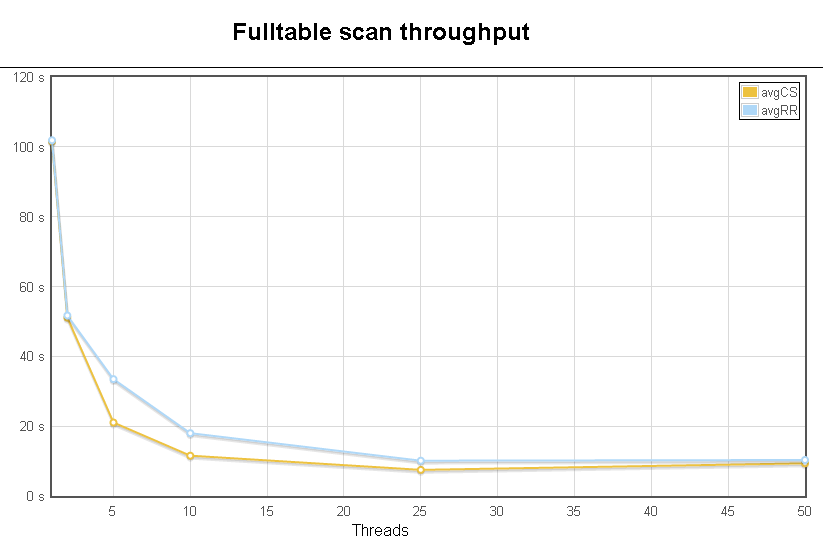
\includegraphics[width=10cm]{origtime}
  \caption[Average time over 5 runs]{Average time over 5 runs as a function of
  swap-threads for both Cursor Stability(CS) and Repeatable Read(RR) isolation levels.\\
  We would expect to non-neglible difference between CS and RR but to me it is
  not conclusive in this graph. The runtime is improved on increased parallelism
  for both isolation levels}\label{fig:origtime}
\end{figure}

Figure \ref{fig:origtime} shows the average runtime(y-axis) for 5 runs by run.py for
each level of concurrency (x-axis).

\begin{figure}
  \centering
  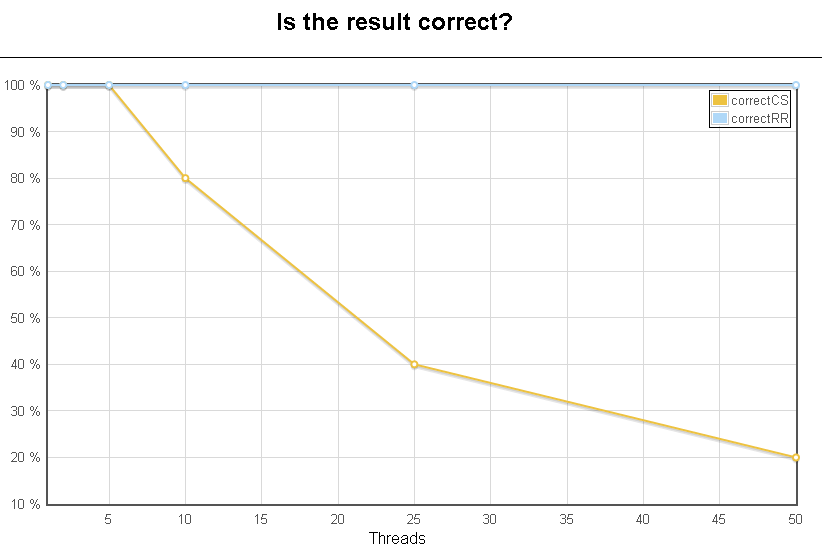
\includegraphics[width=10cm]{origcorrect}
  \caption{Average time over 5 runs as a function of swap-threads.}\label{fig:origcorrect}
\end{figure}

\section{Additional experiment}\label{sec:add}

%\begin{figure}
%\end{figure}


\chapter{Currently Committed}\label{sec:curcommit}
\ldots


\end{document}
